% Copyright (C) 2013 - Michael Baudin
%
% This file must be used under the terms of the 
% Creative Commons Attribution-ShareAlike 3.0 Unported License :
% http://creativecommons.org/licenses/by-sa/3.0/

    \chapter{The Van Der Corput sequence}

\section{Introduction}

      Let $k\geq 0$ be an integer and let b be a prime number.
      We decompose k into base b:
$$
        k=a_{r-1}(k) b^{r-1} + ...+ a_2(k) b^2 + a_1(k) b + a_0(k)
$$
      where r is the number of digits required in the decomposition.

      We can also write this decomposition as the sum:

$$
        k=\sum_{i=0}^{r-1} a_i(k) b^i.
$$

      In order to write the decomposition of an 
	  integer in base b, some authors write:
$$
        k=(a_{r-1}...a_2 a_1 a_0)_b
$$

      The radical inverse function is
$$
        \psi_b(k)=\sum_{i=0}^{r-1} a_{i}(k)b^{-i-1}.
$$

      This can be expanded in:
$$
        \psi_b(k)=a_0(k)b^{-1} + a_1(k)b^{-2} + .. + a_{r-1}(k)b^{-r}.
$$

      This can also be written:
$$
        k=(0.a_0 a_1 a_2 ... a_{r-1})_b
$$

      In this function, the least significant digits of k (with small values of i)
      are in the most significant digits of the radical inverse
      (with small values of powers of 1/b).

      The base-b Van Der Corput sequence is 
$$
        x_i=\psi_b(i), \qquad i \geq 0.
$$

      Notice that
$$
        \psi_b(0)=0.
$$

\section{Van Der Corput sequence in base 2}

      The Van Der Corput sequence in base 2 is just the first component
      of the Halton sequence.
      The following script considers the numbers k from
      zero to 9, decompose them in base 2 and compute the
      k-th element of the Van Der Corput sequence in base 2.

\lstset{language=scilabscript}
\begin{lstlisting}
b=2;
n=b^4;
u=lowdisc_ldgen(n,1,"halton");
for k=1:n
    d=number_tobary(k,b);
    dstr=strcat(string(d),"");
    drev=strcat(string(d($:-1:1)),"");
    mprintf("k=%d=(%s)_%d, r=(0.%s)_%d=%f\n",..
    k,dstr,b,drev,b,u(k,1))
end
   \end{lstlisting}


      The previous script produces the following output.


\lstset{language=scilabscript}
\begin{lstlisting}
k=1=(1)_2, r=(0.1)_2=0.500000
k=2=(10)_2, r=(0.01)_2=0.250000
k=3=(11)_2, r=(0.11)_2=0.750000
k=4=(100)_2, r=(0.001)_2=0.125000
k=5=(101)_2, r=(0.101)_2=0.625000
k=6=(110)_2, r=(0.011)_2=0.375000
k=7=(111)_2, r=(0.111)_2=0.875000
k=8=(1000)_2, r=(0.0001)_2=0.062500
k=9=(1001)_2, r=(0.1001)_2=0.562500
k=10=(1010)_2, r=(0.0101)_2=0.312500
k=11=(1011)_2, r=(0.1101)_2=0.812500
k=12=(1100)_2, r=(0.0011)_2=0.187500
k=13=(1101)_2, r=(0.1011)_2=0.687500
k=14=(1110)_2, r=(0.0111)_2=0.437500
k=15=(1111)_2, r=(0.1111)_2=0.937500
k=16=(10000)_2, r=(0.00001)_2=0.031250
   \end{lstlisting}


      For example, the integer k=6 decomposes as 110 in base 2, because
      $2^2+2^1=4+2=6$.
      Its radical inverse is 0.011 in base 2, which is associated to
      the radical inverse value $0/2+1/4+1/8=0.375$.



      The figure \ref{fig-vdc-base2} plots the points of the Van Der Corput 
	  sequence in base 2.

\begin{figure}[htbp]
\begin{center}
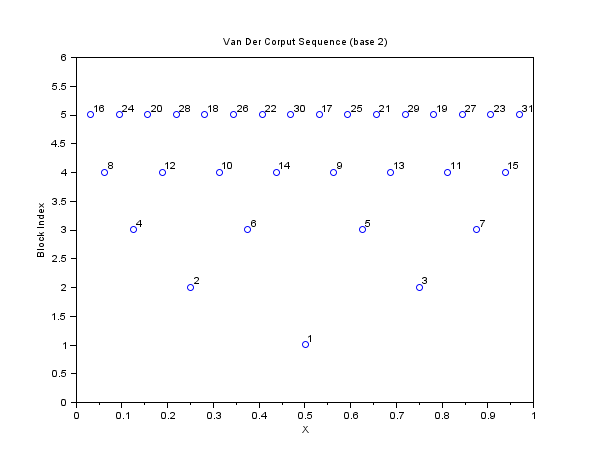
\includegraphics[width=15cm]{figures/vandercorput-base2.png}
\end{center}
\caption{The Van Der Corput sequence in base 2.}
\label{fig-vdc-base2}
\end{figure}

      In base 2, the lowest order digits are alternatively 0, 1, 0, etc... 
	  The most significant digit of the radical inverse function is alternatively 
	  0, 1, 0, etc...
      Hence, the radical inverse in base 2 is alternatively lower 
      and greater than 1/2. 
	  This can be seen in the plot, where the even points are on the 
	  left of the figure, while the odd points are on the right of the 
	  figure.



      Another property which is made clear from the figure is that the 
	  interval [0,1] is progressively filled block-by-block, where 
	  each block of points has an increasing size which is a power of 2. 
	  Indeed, the first block has size 1 (the point 1), the second block has 
	  size 2 (the points 2 and 3), the third block has size 4 (the points 
	  4 to 7), and so on. 
      Therefore, when we use a point set which is a power of two, 
	  we have a regular discretization of the [0,1] interval. 

	  <title>Van Der Corput sequence in base 3</title>

      To get the Van Der Corput sequence in base 3, we just use
      the second dimension of the Halton sequence in two dimensions.


\lstset{language=scilabscript}
\begin{lstlisting}
    b=3;
    n=b^3;
    u=lowdisc_ldgen(n,2,"halton");
    for k=1:n
        d=number_tobary(k,b);
        dstr=strcat(string(d),"");
        drev=strcat(string(d($:-1:1)),"");
        mprintf("k=%d=(%s)_%d, r=(0.%s)_%d=%f\n",..
        k,dstr,b,drev,b,u(k,2))
    end
   \end{lstlisting}


      The previous script produces the following output.


\lstset{language=scilabscript}
\begin{lstlisting}
k=1=(1)_3, r=(0.1)_3=0.333333
k=2=(2)_3, r=(0.2)_3=0.666667
k=3=(10)_3, r=(0.01)_3=0.111111
k=4=(11)_3, r=(0.11)_3=0.444444
k=5=(12)_3, r=(0.21)_3=0.777778
k=6=(20)_3, r=(0.02)_3=0.222222
k=7=(21)_3, r=(0.12)_3=0.555556
k=8=(22)_3, r=(0.22)_3=0.888889
k=9=(100)_3, r=(0.001)_3=0.037037
k=10=(101)_3, r=(0.101)_3=0.370370
k=11=(102)_3, r=(0.201)_3=0.703704
k=12=(110)_3, r=(0.011)_3=0.148148
k=13=(111)_3, r=(0.111)_3=0.481481
k=14=(112)_3, r=(0.211)_3=0.814815
k=15=(120)_3, r=(0.021)_3=0.259259
k=16=(121)_3, r=(0.121)_3=0.592593
k=17=(122)_3, r=(0.221)_3=0.925926
k=18=(200)_3, r=(0.002)_3=0.074074
k=19=(201)_3, r=(0.102)_3=0.407407
k=20=(202)_3, r=(0.202)_3=0.740741
k=21=(210)_3, r=(0.012)_3=0.185185
k=22=(211)_3, r=(0.112)_3=0.518519
k=23=(212)_3, r=(0.212)_3=0.851852
k=24=(220)_3, r=(0.022)_3=0.296296
k=25=(221)_3, r=(0.122)_3=0.629630
k=26=(222)_3, r=(0.222)_3=0.962963
k=27=(1000)_3, r=(0.0001)_3=0.012346
   \end{lstlisting}


      For example, the integer k=6 decomposes as 20 in base 3.
      Its radical inverse is 0.02 in base 3, which is associated to
      the radical inverse value 2/9=0.2222...



      The figure \ref{fig-vdc-base3} plots the points of the Van Der Corput 
	  sequence in base 3.

\begin{figure}[htbp]
\begin{center}
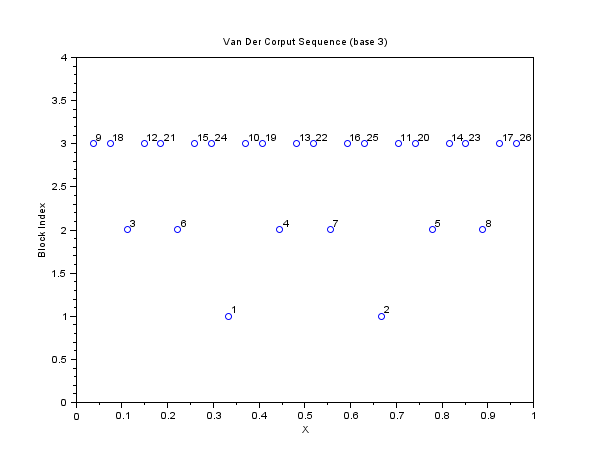
\includegraphics[width=15cm]{figures/vandercorput-base3.png}
\end{center}
\caption{The Van Der Corput sequence in base 3.}
\label{fig-vdc-base3}
\end{figure}

      We see that the [0,1] interval is regularily discretized when 
	  we consider a number of points which is either 3-1=2, 9-1=8 
	  or 27-1=26 points. 
	  In other words, when the number of points is a power of the 
	  base (which is here equal to 3), then the interval is filled 
	  more regularly.

	

      The figure \ref{fig-vdc-base5} plots the points of the Van Der Corput 
	  sequence in base 5.

\begin{figure}[htbp]
\begin{center}
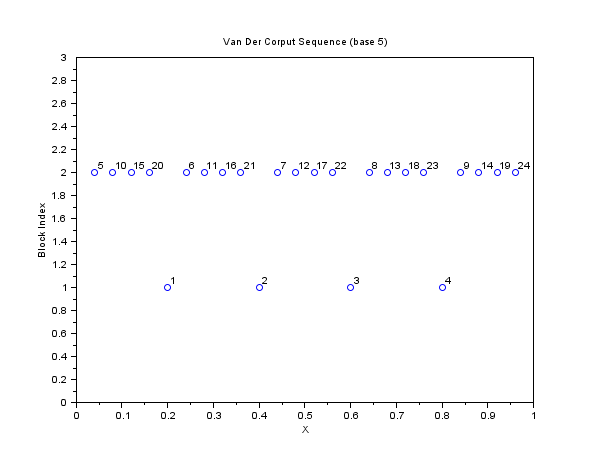
\includegraphics[width=15cm]{figures/vandercorput-base5.png}
\end{center}
\caption{The Van Der Corput sequence in base 5.}
\label{fig-vdc-base5}
\end{figure}

      When the base increases, the number of points before the
      [0,1] interval is regularly filled increases rapidly (as a power of b). 


      Moreover, consider the points 5 to 9, then 10 to 14 : they
      progressively go from left to right, taking b=5 iterations
      to make a partial circle.
      More generally, the subsequences take more iterations to go from lower values (near 0)
      to larger values (near 1).
      This is because it takes b iterations for the the least significant digits
      to go from 0 to b-1.


\section{Properties}

	  The Van Der Corput sequence is a (0,1)-sequence.    
	  Hence, for any $m \geq 0$, consider the point set with 
	  indices $kb^m,...,(k+1)b^m-1$, 
	  for k=0,1,...,b-1. 
      Then, any elementary interval of length $1/b^m$ contains 
	  exactly one point. 
	  For m=0, this just implies that the points are in the [0,1] interval. 

	  In the following script, we consider the Van Der Corput point sets for the 
	  base b=5. 
	  This is just the third dimension of the Halton sequence. 
	  For m=1, we consider the previously defined point sets and plot the 
	  limits of the intervals of length $1/b^m$. 
	  Then we plot the point sets, for k=0,1,...,b-1. 

	
\lstset{language=scilabscript}
\begin{lstlisting}
s=3;
b=5;
m=1;
u=lowdisc_ldgen(b^(m+1),s,"halton");
u=[zeros(1,s);u];
u=u(:,s);
scf();
// Plot the limits
for i=1:b^m
    x=i/b^m;
    plot([x x],[0 b-1],"r-")
end
// Plot the point sets
for k=0:b-1
    indices=k*b^m+1:(k+1)*b^m;
    plot(u(indices)',k,"bo")
    xstring(u(indices)',k,string(indices))
end
a = gca();
a.data_bounds=[
0 -0.5
1 b-0.5
];
a.isoview="off";
st=msprintf("Van Der Corput Sequence, Base %d, %d Points",b,b^(m+1));
xtitle(st,"X","Block Index")
   \end{lstlisting}
	

	  The previous script produces the figure \ref{fig-vandercorput-b5-n25}. 
	  We check that each point set has exactly one point in each 
	  elementary interval, with the convention that the intervals 
	  are closed on the left and open on the right.

\begin{figure}[htbp]
\begin{center}
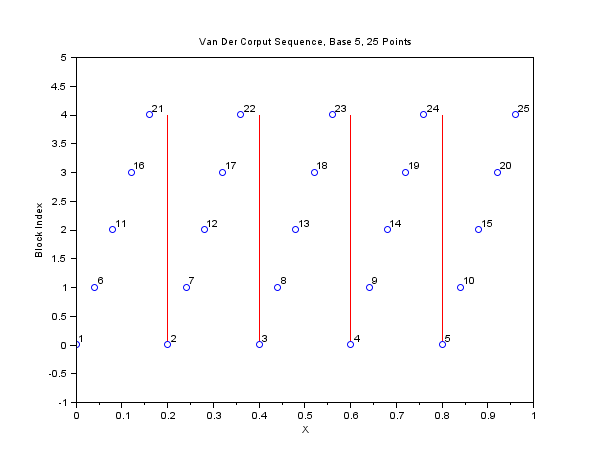
\includegraphics[width=15cm]{figures/vandercorput-b5-n25.png}
\end{center}
\caption{The Van Der Corput sequence in base 5 - 25 points.}
\label{fig-vandercorput-b5-n25}
\end{figure}



	  When we set $s=1$ and $b=2$, 
	  we get the Van Der Corput sequence in base b=2, 
	  which is presented in the figures \ref{fig-vandercorput-b2-n4}, 
	  \ref{fig-vandercorput-b2-n8} and \ref{fig-vandercorput-b2-n16}.

\begin{figure}[htbp]
\begin{center}
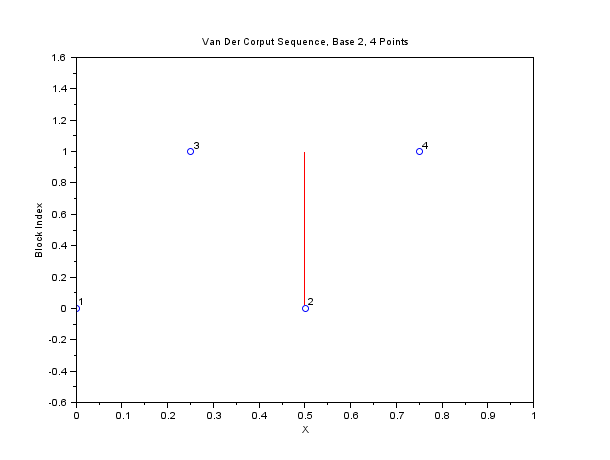
\includegraphics[width=13cm]{figures/vandercorput-b2-n4.png}
\end{center}
\caption{The Van Der Corput sequence in base 2 - 4 points.}
\label{fig-vandercorput-b2-n4}
\end{figure}

\begin{figure}[htbp]
\begin{center}
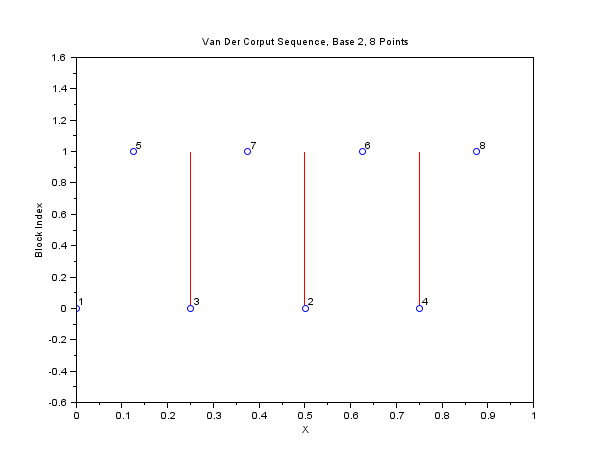
\includegraphics[width=13cm]{figures/vandercorput-b2-n8.png}
\end{center}
\caption{The Van Der Corput sequence in base 2 - 8 points.}
\label{fig-vandercorput-b2-n8}
\end{figure}

\begin{figure}[htbp]
\begin{center}
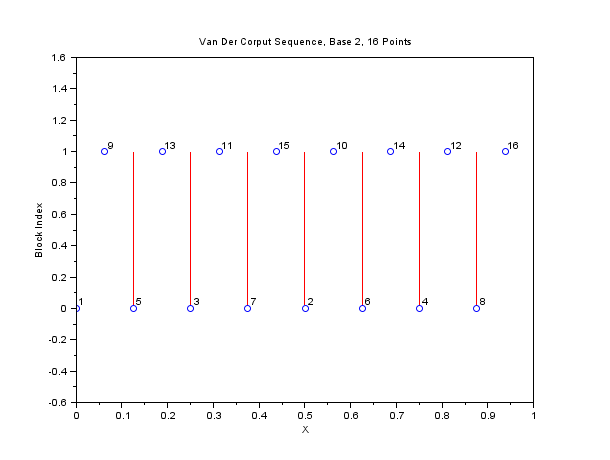
\includegraphics[width=13cm]{figures/vandercorput-b2-n16.png}
\end{center}
\caption{The Van Der Corput sequence in base 2 - 16 points.}
\label{fig-vandercorput-b2-n16}
\end{figure}

\section{Example}

In this section, we present an exemple which shows how particular 
segments of the Van Der Corput behave. 
These segments are chosen so that they match the properties 
of $(t,s)$-sequences. 

Let $m,k\geq 0$ be two integers, let $b$ be 
a prime number and consider the 
elements on the Van Der Corput sequence in base $b$ 
with indices $i=kb^m,...,(k+1)b^m-1$. 
The following script presents the Van Der Corput 
sequence in base $b=2$ and considers $m=5$ and $k=13$. 
We first decompose the integer $i$ into base $b=2$. 

\lstset{language=scilabscript}
\begin{lstlisting}
b=2;
m=5;
u=lowdisc_ldgen(1000,1,"halton");
k=13;
for i=k*b^m:(k+1)*b^m-1
    d=number_tobary(i,b)';
    mprintf("i=%d=(%s)\n",i,strcat(string(d),","))
end
\end{lstlisting}

The previous script produces the following output. 
\lstset{language=scilabscript}
\begin{lstlisting}
i=416=(1,1,0,1,0,0,0,0,0)
i=417=(1,1,0,1,0,0,0,0,1)
i=418=(1,1,0,1,0,0,0,1,0)
i=419=(1,1,0,1,0,0,0,1,1)
i=420=(1,1,0,1,0,0,1,0,0)
[...]
i=443=(1,1,0,1,1,1,0,1,1)
i=444=(1,1,0,1,1,1,1,0,0)
i=445=(1,1,0,1,1,1,1,0,1)
i=446=(1,1,0,1,1,1,1,1,0)
i=447=(1,1,0,1,1,1,1,1,1)
\end{lstlisting}

We see that the 9 bits are required to decompose these 
integers into base 2. 
The four first bits are $(1,1,0,1)$, which 
is explained by the fact that $k=13=2^3+2^2+2^0$. 
The bits from 5 to 9 are all the possible bits in the set $\{0,1\}$. 

Then we decompose the i-th element of the Van Der Corput sequence 
\scivar{u(i)} into base $b=2$, printing the first 10 digits 
(the remaining low order digits are all zero).

\lstset{language=scilabscript}
\begin{lstlisting}
for i=k*b^m:(k+1)*b^m-1
    d=flps_tobary(u(i),b,10)';
    mprintf("u(i)=%f=(%s)\n",u(i),strcat(string(d),","))
end
\end{lstlisting}

The previous script produces the following output. 

\lstset{language=scilabscript}
\begin{lstlisting}
u(416)=0.021484375=(0,0,0,0,0,0,1,0,1,1)
u(417)=0.521484375=(0,1,0,0,0,0,1,0,1,1)
u(418)=0.271484375=(0,0,1,0,0,0,1,0,1,1)
u(419)=0.771484375=(0,1,1,0,0,0,1,0,1,1)
[...]
u(444)=0.240234375=(0,0,0,1,1,1,1,0,1,1)
u(445)=0.740234375=(0,1,0,1,1,1,1,0,1,1)
u(446)=0.490234375=(0,0,1,1,1,1,1,0,1,1)
u(447)=0.990234375=(0,1,1,1,1,1,1,0,1,1)
\end{lstlisting}

For example, the decomposition of 0.521484375 is 
$1/2+1/2^6+1/2^8+1/2^9$.

We see that the 4 low order bits are $(1,0,1,1)$, 
which are the reverse bits of the decomposition of $k$. 
The bits from 2 to 6 are all the possible bits in the set $\{0,1\}$. 

\section{Property}

\begin{proposition}
\label{vdc-01net}
The Van Der Corput sequence is a $(0,1)$-sequence.
\end{proposition}

\begin{proof}
Let a be an integer in the set $\{0,1,...,b^m-1\}$.
Let $I=[a/b^m,(a+1)/b^m)$ be an elementary interval. 
Its length is $1/b^m$. 
Let $k \geq 0$ be an integer. 
Let us prove that there is a unique $i$ in the set $\{kb^m,...,(k+1)b^m-1\}$  
such that $\phi(i) \in I$, where $\phi(i)$ is the i-th element 
of the Van Der Corput sequence in base $b$.
Let $a(0),a(1),...,a(m-1) \in \{0,1,...,b-1\}$ be the $m$ digits 
of the base-b decomposition of a:
\begin{eqnarray}
a=a(0) b^{m-1}+...+a(m-2) b+a(m-1).
\end{eqnarray}
Notice that the digits are ordered from the highest to the lowest 
significant digits. 
Let $a(m),a(m+1),...,a(m+r-1) \in \{0,1,...,b-1\}$ be the 
$r$ digits of the base-b decomposition of $k$ in base $b$:
\begin{eqnarray}
k=a(m+r-1)b^{r-1}+...+a(m+1)b+a(m). \label{vdc-01netdefk}
\end{eqnarray}
Notice that the digits are ordered from the lowest to the highest 
significant digits.
Let us introduce:
\begin{eqnarray}
t&=&\frac{a}{b^m} \\
 &=&\frac{a(0)}{b}+\frac{a(1)}{b^2}+...+\frac{a(m-1)}{b^m} \\
\end{eqnarray}
and
\begin{eqnarray}
x&=&\frac{a(m)}{b}+\frac{a(m+1)}{b^2}+...+\frac{a(m+r-1)}{b^r}.
\end{eqnarray}
Notice that $t$ is uniquely defined from the digits arising from the 
base-b decomposition of $a$ while $x$ is uniquely defined from the digits 
arising from the base-b decomposition of $k$. 
Consider the number 
\begin{eqnarray}
y&=&t+\frac{x}{b^m} \\
 &=&\frac{a(0)}{b}+\frac{a(1)}{b^2}+...+\frac{a(m-1)}{b^m} \nonumber \\
  &&+\frac{a(m)}{b^{m+1}}+\frac{a(m+1)}{b^{m+2}}+...+\frac{a(m+r-1)}{b^{m+r}}
  \label{vdc-01netdefy}
\end{eqnarray}
Obviously $x\geq 0$. 
Moreover, 
\begin{eqnarray}
x &\leq& \frac{b-1}{b}+\frac{b-1}{b^2}+...+\frac{b-1}{b^r} \\
  &   <& 1.
\end{eqnarray}
Indeed, this is a geometric series:
\begin{eqnarray}
\frac{b-1}{b}+\frac{b-1}{b^2}+...+\frac{b-1}{b^r}
&=& \frac{b-1}{b}(1+\frac{1}{b}+\frac{1}{b^2}+...+\frac{1}{b^{r-1}} \\
&=& \frac{b-1}{b} \frac{1-\frac{1}{b^r}}{1-\frac{1}{b}} \\
&=& \frac{b-1}{b} \frac{1-\frac{1}{b^r}}{\frac{b-1}{b}} \\
&=& 1-\frac{1}{b^r} \\
&<& 1.
\end{eqnarray}
Therefore, $x \in [0,1)$. 
Hence, $a+x \in [a,a+1)$ so that $a/b^m+x/b^m \in I$. 
But $t=\frac{a}{b^m}$, which implies $t+x/b^m=y \in I$. 
In order to conclude the proof, we recognize that $y$ 
is the i-th element of the Van Der Corput sequence in base b, 
for a particular value of $i$. 
To see this value of $i$, we just reverse the digits 
of the definition of $y$ from the equation \ref{vdc-01netdefy}. 
This leads to 
\begin{eqnarray}
i &=& a(m+r-1) b^{m+r-1}+...+a(m+1) b^{m+1}+a(m) b^m \nonumber \\
  & & a(m-1)b^{m-1}+...+a(1)b+a(0) \\
  &=& \left( a(m+r-1) b^{r-1}+...+a(m+1) b+a(m)\right) b^m \nonumber \\
  & & a(m-1)b^{m-1}+...+a(1)b+a(0) \\
  &=& kb^m+a(m-1)b^{m-1}+...+a(1)b+a(0),
\end{eqnarray}
where the last equality is implied by the equation \ref{vdc-01netdefk}.
Moreover, 
$$
0\leq a(m-1) b^{m-1}+...+a(1) b+a(0) \leq b^m-1. 
$$
Hence 
$$
k b^m \leq i \leq kb^m+b^m-1=(k+1)b^m-1.
$$
We have computed the unique i such that 
$y=\phi(i)$ is in I, which concludes the proof. 
\end{proof}
